
\subsection*{Общая характеристика работы}

\newcommand{\actuality}{\underline{\textbf{\actualityTXT}}}
\newcommand{\progress}{\underline{\textbf{\progressTXT}}}
\newcommand{\aim}{\underline{{\textbf\aimTXT}}}
\newcommand{\tasks}{\underline{\textbf{\tasksTXT}}}
\newcommand{\novelty}{\underline{\textbf{\noveltyTXT}}}
\newcommand{\influence}{\underline{\textbf{\influenceTXT}}}
\newcommand{\methods}{\underline{\textbf{\methodsTXT}}}
\newcommand{\defpositions}{\underline{\textbf{\defpositionsTXT}}}
\newcommand{\reliability}{\underline{\textbf{\reliabilityTXT}}}
\newcommand{\probation}{\underline{\textbf{\probationTXT}}}
\newcommand{\contribution}{\underline{\textbf{\contributionTXT}}}
\newcommand{\publications}{\underline{\textbf{\publicationsTXT}}}

{\actuality} 
% Актуальность - необходимо уметь контролировать рассеяние и поглощение,
% есть невидимость. Добавить 5 ссылок. Актуально сделать маскирующие
% покрытие на основе диэлектриков. 

В последние годы появилось большое количество работ по
нанофотонике~\cite{Tame-quantum-plasmonics-2013,
  Javier-graphene-plasmonics-2014, Khurgin-loss-plasmonics-2015,
  He-tunable-terahertz-graphene-metamaterials-2015,
  Segal-meta-nonlinar-PhC-2015,
  Poddubny-hyperbolic-metamaterials-2013, Kildishev-metasurface-2013}.
Высокая актуальность полученных результатов связана с перспективами их
практического применения и обусловлена стремительным развитием
нанотехнологий, что даёт возможность экспериментальной проверки
предлагаемых идей и подходов. Среди прочих, стоит отметить вопрос о
взаимодействии света с многослойной сферической наночастицей. Он
рассматривается в ряде прикладных задач, таких как: лечение
рака~\cite{Zhang-2010, Hirsch-2003}, различные методы диагностики в
медицине~\cite{Allain-2002}, разработка маскирующих суб-волновых
покрытий для видимого и микроволнового диапазонов~\cite{Qui-2009,
  Semouchkina-2013}, устройства плазмоники~\cite{Martin-2013,
  Alu-2005}, изучение тепловых свойств изоляторов~\cite{Xie-2013},
повышение эффективности солнечных элементов~\cite{Kameya-2011,
  Mann-2011} и так далее. Всё вместе это обуславливает актуальность
настоящей работы, в которой сперва излагается общий принцип,
позволяющий управлять рассеянием и поглощением электромагнитных волн
многослойными сферическими наночастицами, а потом идёт апробация на
частных примерах: минимизация рассеяния от идеально проводящей сферы
(частичная невидимость) и управление поглощением плазмонной частицы
$Si/Ag/Si$.

\underline{\textbf{Основные методы исследования.}}
Теория Ми~\cite{Mie-1908} входит в число основных инструментов применяемых
при анализе задач рассеяния и поглощения плоской электромагнитной
волны сферическими объектами. Эта теория была обобщённа на случай
многослойной сферы с произвольным числом слоёв~\cite{Yang-2003,
  Pena-scattnlay-2009} и доработана в настоящей работе, что позволило
реализовать её в виде комплекса программ для проведения компьютерного
моделирования. Достоинством теории является используемое ей разложение
поля по сферическим векторным гармоникам, что позволяет разделить
вклад в общее поле от электрического и магнитного дипольного
резонанса, а так же вклад резонансов квадруполя
и мультиполей более высокого порядка. Таким образом, становится
возможен анализ спектрального отклика многослойной сферы в зависимости
от её параметров (размеров и показателей преломления слоёв). Например,
в ряде случаев удаётся совместить в спектре рассеяния положение
нескольких резонансов (например, электрических дипольного и
квадрупольного), что создаёт эффект
суперрассеяния~\cite{Fan-2010,Fan-2011}. Аналогичный эффект
суперпоглощения подробно рассмотрен в настоящей работе.


 Как правило, при их решении возникает
необходимость оптимизации дизайна многослойной сферы (радиусов и
материальных параметров составных слоёв), обеспечивающего наилучшие
рабочие характеристики для каждого конкретного случая с учётом
фактических ограничений в предметной области.


\aim\ данной работы является разработка общего подхода к оптимизации
дизайнов многослойных сфер в рамках теории Ми, его последующая
реализация в комплексе компьютерных программ, выявление
закономерностей между дизайном многослойной сферы и её оптическими
свойствами.

Для~достижения поставленной цели необходимо было решить следующие {\tasks}:
\begin{enumerate}
  \item Разработать алгоритм для вычисления рассеяния и поглощения в
    многослойных сферических объектах и реализовать его в комплексе программ.
  \item Выбрать и реализовать алгоритм оптимизации, подходящий для
    работы с произвольными параметрами модели, описываемой обобщённой
    теорией Ми.
  \item Выявить основные закономерности взаимодействия с
    электромагнитной волной сферических маскирующих покрытий на
    основе диэлектриков.
  \item Исследовать эффект суперпоглощения света в многослойных
    сферических наночастицах.
\end{enumerate}



\defpositions
\begin{enumerate}
  \item Получены и реализованны в комплексе программ явные
    реккурентные соотношения для коэффициентов Ми в объёме
    многослойной сферы, выраженные через логарифмические производные
    функций Риккати-Бесселя увеличивающие численную стабильность.  
  
  \item Использование тонкого (размер мишени к размеру покрытия) диэлектриких многослойных покрытий позволяет
    уменьшить рассеяние от идеальное мишени в два раза.
  \item Использовать диэлектрикого порытия для небольшого объекта
    позволяет уменьшить рассеяние в 6 раз.

  \item TODO Использование алгоритма стохастической оптимизации методом
    адаптивной дифференциальной эволюции для решения задачи Ми
    позволяет выявлять семейства дизайнов с заранее заданными
    электромагнитными свойствами.

  \item Защищать цифры (уменьшили в два раза и т.д.). Показано, что
    маскирующие сферические покрытия из диэлектриков могут быть
    сконструированы, используя волноводоподобный эффект.  В этом
    случае при распространении внутри покрытия поле отстает по фазе от
    невозмущённой падающей волны на величину, кратную $2\pi$.
  \item Обнаружено семейство маскирующих сферических порытий из
    диэлектрических изотропных метаматериалов, реализующих эффект
    волнового обтекания.  Для получения заметного эффекта достаточно
    трёх слоёв в покрытии.
  \item В трёхслойных частицах $Si/Ag/Si$ возможно вырождение
    резонансных мультипольных откликов, приводящее к эффекту
    суперпоглощения, когда сечение поглощение оказывается больше, чем
    у bulk частицы. 
  \end{enumerate}

Положения соответствуют пункту 1 паспорта специальности 01.04.05 --
<<Оптика>> (Волновая (физическая) оптика. Интерференция, дифракция,
поляризация, когерентность света) по физико-математическим
наукам (представлены результаты фундаментальных исследований).

%\vspace{5.5em}
\novelty Используем диэлектрики для маскировки, использовать
оптимизация. Есть суперпоглощения.
\begin{enumerate}
  \item Впервые были получены явные реккурентные соотношения для
    коэффициентов Ми в многослойной сфере, выраженные через
    логарифмические производные функций Риккати-Бесселя. 
  \item Впервые метод дифференциальной эволюции был применён
    для изучения маскирующих сферических покрытий, показана высокая
    производительность метода.
  \item Было выполнено оригинальное исследование поглощения света
    наночастицами в режиме вырождения резонансых мультипольных откликов.
\end{enumerate}

\influence. Разработанные аналитические и численные методы для решения
уравнений Максвелла в рамках теории Ми, а так же реализующий их
программный комплекс с использованием стахостической оптимизации
методом дифференциальной эволюции могут быть использованы при
проектировании, оптимизации и анализе (включая анализ предельно
достижимых рабочих характеристик) широкого спектра устройств,
работающих как в оптическом, так и микроволновом диапазоне. Результаты
полученные при изучении поглощени света наночастицами могут быть
использованы при разработке инновационных устройств наноплазмоники,
фотоактивных катализаторов, красителей, поглощающих эмульсий и
аэрозолей.

Результаты диссертационной работы использовались при выполнении
грантов Министерства образования и науки РФ
(проект 11.G34.31.0020, гос. задание 2014/190, задание 3.561.2014/K),
Правительства РФ (грант 074-U01), РФФИ (грант 15-57-45141 ИНД\verb+_+а).


\reliability\ полученных результатов обеспечивается методическим
подходом на каждом этапе работы. Работа оптимизатора была проверена на
наборе стандартных тестовых функций. Аналитические результаты работы
были проверены в системе компьютерной алгебры (IPython). Компьютерная
реализация решения была проверена на наборе тестовых
задач. Аналитические результаты находятся в соответствии с
результатами, полученными другими авторами по теории Ми для случаев
однородной сферы и сферы с одним слоем покрытия.  Случаи большего
числа слоёв в покрытии сравнивался с коммерческими пакетами
моделирования, использующих численные методы конечных разностей во
временной области (Lumerical FDTD), метод конечных элементов (Comsol)
и метод конечных интегралов (CST MWS). Результаты по исследованию
маскирующих покрытий и поглощения света наночастицами находятся в
соответствии с результатами, полученными другими авторами для похожих
систем.

\probation\
Основные результаты работы докладывались~на:
перечисление основных конференций, симпозиумов и~т.\:п.

\contribution\ Автор принимал активное участие \ldots

%\publications\ Основные результаты по теме диссертации изложены в ХХ печатных изданиях~\cite{Sokolov,Gaidaenko,Lermontov,Management},
%Х из которых изданы в журналах, рекомендованных ВАК~\cite{Sokolov,Gaidaenko}, 
%ХХ --- в тезисах докладов~\cite{Lermontov,Management}.
 
\ifthenelse{\equal{\thebibliosel}{0}}{% Встроенная реализация с загрузкой файла через движок bibtex8
    \publications\ Основные результаты по теме диссертации изложены в XX печатных изданиях, 
    X из которых изданы в журналах, рекомендованных ВАК, 
    X "--- в тезисах докладов.%
}{% Реализация пакетом biblatex через движок biber
%Сделана отдельная секция, чтобы не отображались в списке цитированных материалов
    \begin{refsection}%
        \printbibliography[heading=countauthornotvak, env=countauthornotvak, keyword=biblioauthornotvak, section=1]%
        \printbibliography[heading=countauthorvak, env=countauthorvak, keyword=biblioauthorvak, section=1]%
        \printbibliography[heading=countauthorconf, env=countauthorconf, keyword=biblioauthorconf, section=1]%
        \printbibliography[heading=countauthor, env=countauthor, keyword=biblioauthor, section=1]%
        \publications\ Основные результаты по теме диссертации изложены в \arabic{citeauthor} печатных изданиях\nocite{bib1,bib2}, 
        \arabic{citeauthorvak} из которых изданы в журналах, рекомендованных ВАК\nocite{Ladutenko-cloak-2014,Ladutenko-Qabs-2015}, 
        \arabic{citeauthorconf} "--- в тезисах докладов\nocite{DD-14, MW-14}.%
    \end{refsection}
}
% При использовании пакета \verb!biblatex! для автоматического подсчёта
% количества публикаций автора по теме диссертации, необходимо
% их здесь перечислить с использованием команды \verb!\nocite!.
    

 % Характеристика работы по структуре во введении и в автореферате не отличается (ГОСТ Р 7.0.11, пункты 5.3.1 и 9.2.1), потому её загружаем из одного и того же внешнего файла, предварительно задав форму выделения некоторым параметрам

%Диссертационная работа была выполнена при поддержке грантов ...

%\underline{\textbf{Объем и структура работы.}} Диссертация состоит из~введения, четырех глав, заключения и~приложения. Полный объем диссертации \textbf{ХХХ}~страниц текста с~\textbf{ХХ}~рисунками и~5~таблицами. Список литературы содержит \textbf{ХХX}~наименование.

%\newpage
\subsection*{Содержание работы}
Во \underline{\textbf{введении}} обосновывается актуальность
исследований, проводимых в рамках данной диссертационной работы,
приводится обзор научной литературы по изучаемой проблеме,
формулируется цель, ставятся задачи работы, сформулированы научная
новизна и практическая значимость представляемой работы. В последующих
главах сперва излагается общий принцип, позволяющий управлять
поглощением и рассеянием электромагнитных волн от многослойной
сферической наночастицы, а потом идёт апробация на частных примерах:
минимизация рассеяния от идеально-проводящей сферы (случай частичной
невидимости, т.е. маскировки объекта) и управление поглощением в плазмонной
частице $Si/Ag/Si$.


\underline{\textbf{Первая глава}} посвящена модификации теории Ми для
случая многослойной сферы. 

Более 100 лет назад Густав Ми опубликовал свою оригинальную
работу~\cite{Mie-1908} о взаимодействии плоской электромагнитной волны
с однородной сферой.  Изложенная в ней теория впоследствии получила
его имя и в настоящее время входит в число основных инструментов
применяемых при анализе задач рассеяния и поглощения сферическими
объектами.  Несмотря на более чем вековую историю теории Ми, работы по
её дальнейшему развитию ведутся и в настоящее время% ~\cite{Suzuki-2008,
% MacKowski-2012, Lerme-2000, Xu-2005, Li-2006, Gogoi-2010,
% Santiago-2011}
.  Рядом авторов были предложены математические
модели~\cite{Yang-2003, Pena-scattnlay-2009}, позволяющие изучать
многослойные сферы с произвольным числом слоёв.  Основная сложность
при этом возникает при численной реализации этих моделей.  В теории Ми
решение для рассеянного поля выражается в виде разложения в ряд:
\begin{align*}
{\rm \mathbf{E}}_s &=\sum_{n=1}^{\infty} E_n \left( i a_n {\rm
    \mathbf{N}}_{e1n}^{(3)} - b_n{\rm\mathbf{M}_{o1n}^{(3)}} \right)\\
{\rm \mathbf{H}}_s &=\frac{k}{\omega\mu}
 \sum_{n=1}^{\infty} E_n \left( i b_n {\rm
    \mathbf{N}}_{o1n}^{(3)} + a_n{\rm\mathbf{M}_{e1n}^{(3)}} \right)  
\end{align*}
где $E_n=i^nE_0(2n+1)/n(n+1)$, $n$ порядок мультиполя, $E_0$ амплитуда
падающего поля, $a_n$ и $b_n$ коэффициенты разложения, соответствующие
электирческим и магнитным мультиполям, ${\rm \mathbf{N}}_{e1n}^{(3)}$,
${\rm \mathbf{N}}_{o1n}^{(3)}$, ${\rm\mathbf{M}_{o1n}^{(3)}}$ и
${\rm\mathbf{M}_{e1n}^{(3)}}$ это сферические векторные гармоники,
выражающиеся через тригонометрические функции, полимномы Лежандра и
сферические функции Бесселя и Ханкеля, $k$ и $\omega$ волновой вектор
и частота падающей волны, $\mu$ магнитная проницаемость в вакууме.
Аналогичным образом может быть выражено поле внутри $l$-ого слоя
стратифицированной сферы~\cite{Yang-2003}:
\begin{align}
{\rm \mathbf{E}}_l &=\sum_{n=1}^{\infty} E_n \left(
                     c_n^{(l)}{\rm\mathbf{M}}_{o1n}^{(1)}
                     -i d_n^{(l)} {\rm \mathbf{N}}_{e1n}^{(1)}
                     +i a_n^{(l)} {\rm \mathbf{N}}_{e1n}^{(3)}
                     - b_n^{(l)}{\rm\mathbf{M}}_{o1n}^{(3)} 
                     \right)\label{eq:3p1}\\
{\rm \mathbf{H}}_l &=\frac{k_l}{\omega\mu} \sum_{n=1}^{\infty} E_n
                     \left(
                      d_n^{(l)}{\rm\mathbf{M}}_{e1n}^{(1)} 
                     +i c_n^{(l)} {\rm \mathbf{N}}_{o1n}^{(1)} 
                     -i b_n^{(l)} {\rm \mathbf{N}}_{o1n}^{(3)} 
                     - a_n^{(l)}{\rm\mathbf{M}}_{e1n}^{(3)} 
                     \right)\label{eq:3p2}  
\end{align}
где для каждого слоя определены коэффициенты разложения $d_n^{(l)}$ и
$c_n^{(l)}$ электрического и магнитного поля для входящей волны
(направленной к центру частицы) и, аналогично, $a_n^{(l)}$ и
$b_n^{(l)}$ для исходящей волны.  Связь между всеми коэффициентами
разложения можно выразить в виде системы реккурентных уравнений,
которые получаются из граничных условий между слоями на напрерывность
номальных компонент полей.  Из выражений для падающей
и рассеянной волны получаются дополнительные условия на коэффициенты
разложения $c_n^{(L+1)}=d_n^{(L+1)}=1$, $a_n=a_n^{(L+1)}$ и
$b_n=b_n^{(L+1)}$, где $L$ общее число слоёв. Так как у центального
слоя $l=1$ нет внутренней границы, то
$a_n^{(1)}=b_n^{(1)}=0$. Последнее условие является избыточным и
поэтому оно было использовано для дополнительной проверки
самосогласованности работы компьютерной программы.  После проведения
необходимых алгебраических преобразований значения коэффициентов
разложения были получены явно, в виде обратной реккурентной
последовательности:
\begin{equation}
\label{eq:6p1}
a^{(l)}_n = \frac
{
    {D^{(1)}_{n}}{\left (m_{l} x_{l} \right )}
    T_1\left (m_{l+1} x_{l} \right )
    +
    T_3\left (m_{l+1} x_{l} \right )
    m_{l}/m_{l+1}
}
{
   \zeta_{n}\left (m_{l} x_{l} \right )
   U\left (m_{l} x_{l} \right )
}
\end{equation}
\begin{equation}
\label{eq:6p2}
b^{(l)}_n = \frac
{
    {D^{(1)}_{n}}{\left (m_{l} x_{l} \right )}
    T_2\left (m_{l+1} x_{l} \right )
    m_{l}/m_{l+1}
    +
    T_4\left (m_{l+1} x_{l} \right )
}
{
   \zeta_{n}\left (m_{l} x_{l} \right )
   U\left (m_{l} x_{l} \right )
}
\end{equation}
\begin{equation}
\label{eq:6p3}
c^{(l)}_n = \frac
{
    {D^{(3)}_{n}}{\left (m_{l} x_{l} \right )}
    T_2\left (m_{l+1} x_{l} \right )
    m_{l}/m_{l+1}
    +
    T_4\left (m_{l+1} x_{l} \right )
}
{
   \psi_{n}\left (m_{l} x_{l} \right )
   U\left (m_{l} x_{l} \right )
}
\end{equation}
\begin{equation}
\label{eq:6p4}
d^{(l)}_n = \frac
{
    {D^{(3)}_{n}}{\left (m_{l} x_{l} \right )}
    T_1\left (m_{l+1} x_{l} \right )
    +
    T_3\left (m_{l+1} x_{l} \right )
    m_{l}/m_{l+1}
}
{
   \psi_{n}\left (m_{l} x_{l} \right )
   U\left (m_{l} x_{l} \right )
}
\end{equation}
используя
\begin{equation*}
  U(z) =    {D^{(1)}_{n}}(z) - {D^{(3)}_{n}}(z)
\end{equation*}
\begin{equation*}
  T_1(z) =   a^{(l+1)}_{n}  \zeta_{n}(z) 
           - d^{(l+1)}_{n}  \psi_{n}(z)
\end{equation*}
\begin{equation*}
  T_2(z) =   b^{(l+1)}_{n}  \zeta_{n}(z) 
           - c^{(l+1)}_{n}  \psi_{n}(z)
\end{equation*}
\begin{equation*}
  T_3(z) =  d^{(l+1)}_{n}  D^{(1)}_{n}(z)  \psi_{n}(z) 
          - a^{(l+1)}_{n}  D^{(3)}_{n}(z)  \zeta_{n} (z)
\end{equation*}
\begin{equation*}
  T_4(z) =  b^{(l+1)}_{n}  D^{(1)}_{n}(z)  \psi_{n}(z) 
          - c^{(l+1)}_{n}  D^{(3)}_{n}(z)  \zeta_{n} (z)
\end{equation*}
где $m_l = n_{\rm layer}/n_{\rm host}$ комплексный показатель
преломления в слое, нормированный на показатель преломления
окружающего пространства, $x_l$ параметр размера внешнего радиуса
слоя, $\psi_{n}(z) = z j_n(z)$ и $\zeta_{n}(z) = z h_n^1(z)$ функции
Риккати-Бесселя, выраженные через сферические функции Бесселя и
Ханкеля, $D^{(1)}_{n} = \psi^{\prime}_{n}/\psi_{n}$ и
$D^{(3)}_{n} = \zeta^{\prime}_{n}/\zeta_{n}$ это логарифмические
производные функций Риккати-Бесселя. Подставляя
(\labelcref{eq:6p1,eq:6p2,eq:6p3,eq:6p4}) в уравнения (\ref{eq:3p1}) и
(\ref{eq:3p2}) можно вычислить величину электрического и магнитного
поля внутри и снаружи многослойной сферы. Дополнительно, выразив
сферческие векторные гармоники через логарифмические производные
функций Риккати-Бесселя, удалось заметно увеличить численную
устойчивость вычислений.

Полученные выражения позволили полностью переработать
программу~\cite{Scattnlay-web} для проведения расчёта.  В результате,
программа получила возможность расчёта полей, доработка уже
существоваших алгоритмических решений позволило сократить время
расчёта в 2.2 раза.

\underline{\textbf{Вторая глава}} посвящена выбору универсального
алгоритма оптимизации и вопросам его практической
реализации. Сложность выбора обусловлена огромным количеством методов
оптимизации, а так же большим числом разновидностей каждого
метода. Ряд ограничений, существующий для оптимизации исходных
параметров задачи Ми, позволяет исключить из рассмотрения такие
популярные методы, как метод наискорейшего спуска (требующий
вычисления градиента), симплекс-метод Нелдера--Мида (есть сложность с
локальными экстремумами) и аналогичные им. В результате, приходится
ограничить выбор стахостическими методами, среди которых наиболее
распространёнными являются генетические алгоритмы, методы роя частиц и
методы дифференциальной эволюции.  Все эти алгоритмы используют метод
<<проб и ошибок>>.  Несколько пробных решений (называемых индивидами)
генерируются случайным образом и многократно улучшаются в надежде
найти некое удовлетворительное решение. Качество решения оценивается
целевой функцией, формулируемой в задаче, которую предстоит
оптимизировать.  Полная группа индивидов называется популяцией.
Состояние популяции на конкретном шаге итерации называется поколением.
Переход между поколениями осуществляется в соответствии с рядом
относительно простых правил, которые составляют сущность определённого
алгоритма.

% Генетические алгоритмы обычно рассматривают вещественные числа в виде
% набора битов.  В отличие от них, методы роя частиц и методы
% дифференциальной эволюции могут работать в непрерывном пространстве
% вещественных входных параметров естественным образом (используя
% возможность сложения и вычитания векторов пробных решений), что делает
% их гораздо более удобными для решения физических и инженерных
% задач.  Производительность этих алгоритмов зависит от правильного
% выбора значений некоторых внутренних параметров
% алгоритма.  Использование адаптивных версий алгоритмов упрощает задачу
% оптимизации: их значения внутренних параметров настраиваются
% автоматически при переходе между поколениями. Как правило, адаптивным
% алгоритмам нужно гораздо меньше (более чем на порядок) итераций, чем
% неадаптивным, чтобы добиться того же результата оптимизации.

В настоящей работе был реализован алгоритм JADE+ с улучшенной
скоростью скрещивания (по алгоритму PMCRADE), который является
адаптивным вариантом алгоритма дифференциальной эволюции. Он имеет
явное преимущество перед адаптивной оптимизацией методом роя частиц в
ряде стандартных тестов.  Выполненная в рамках настоящей работы
реализация указанного метода позволяет эффективно использовать
современные процессоры с большим количеством параллельных потоков
вычисления и может выполняться на суперкомпьютерных кластерах, что
стало возможно благодаря использованию программных библиотек,
поддерживающих стандарт Message Parsing Interface (MPI).
Разработанное~\cite{JADE-web} программное обеспечение успешно проходит
набор стандартных тестов для алгоритмов оптимизации.  Было получено
свидетельство о государственной регистрации программы для
ЭВМ~№2014611568.


\underline{\textbf{Третья глава}} посвящена исследованию свойств
многослойных сферических маскирующих покрытий. Схематическое
изображение модели приводится на рисунке~\ref{img:scattering}а. Для
заданного соотношения длины волны и диаметра маскируемого объекта с
помощью оптимизатора подбирались параметры многослойного покрытия
таким образом, чтобы уменьшить полное сечение рассеяния.  Покрытие
разбивалась на фиксированное количество слоёв одинаковой толщины, а в
качестве параметров оптимизации использовались показатели преломления
каждого слоя.  Результат оптимизации в виде зависимости полного
сечения рассеяния от количества слоёв и общей толщины покрытия
приводится на рисунке~\ref{img:scattering}б.
\begin{figure}[t]
  \begin{minipage}[ht]{0.45\linewidth}        
    \center{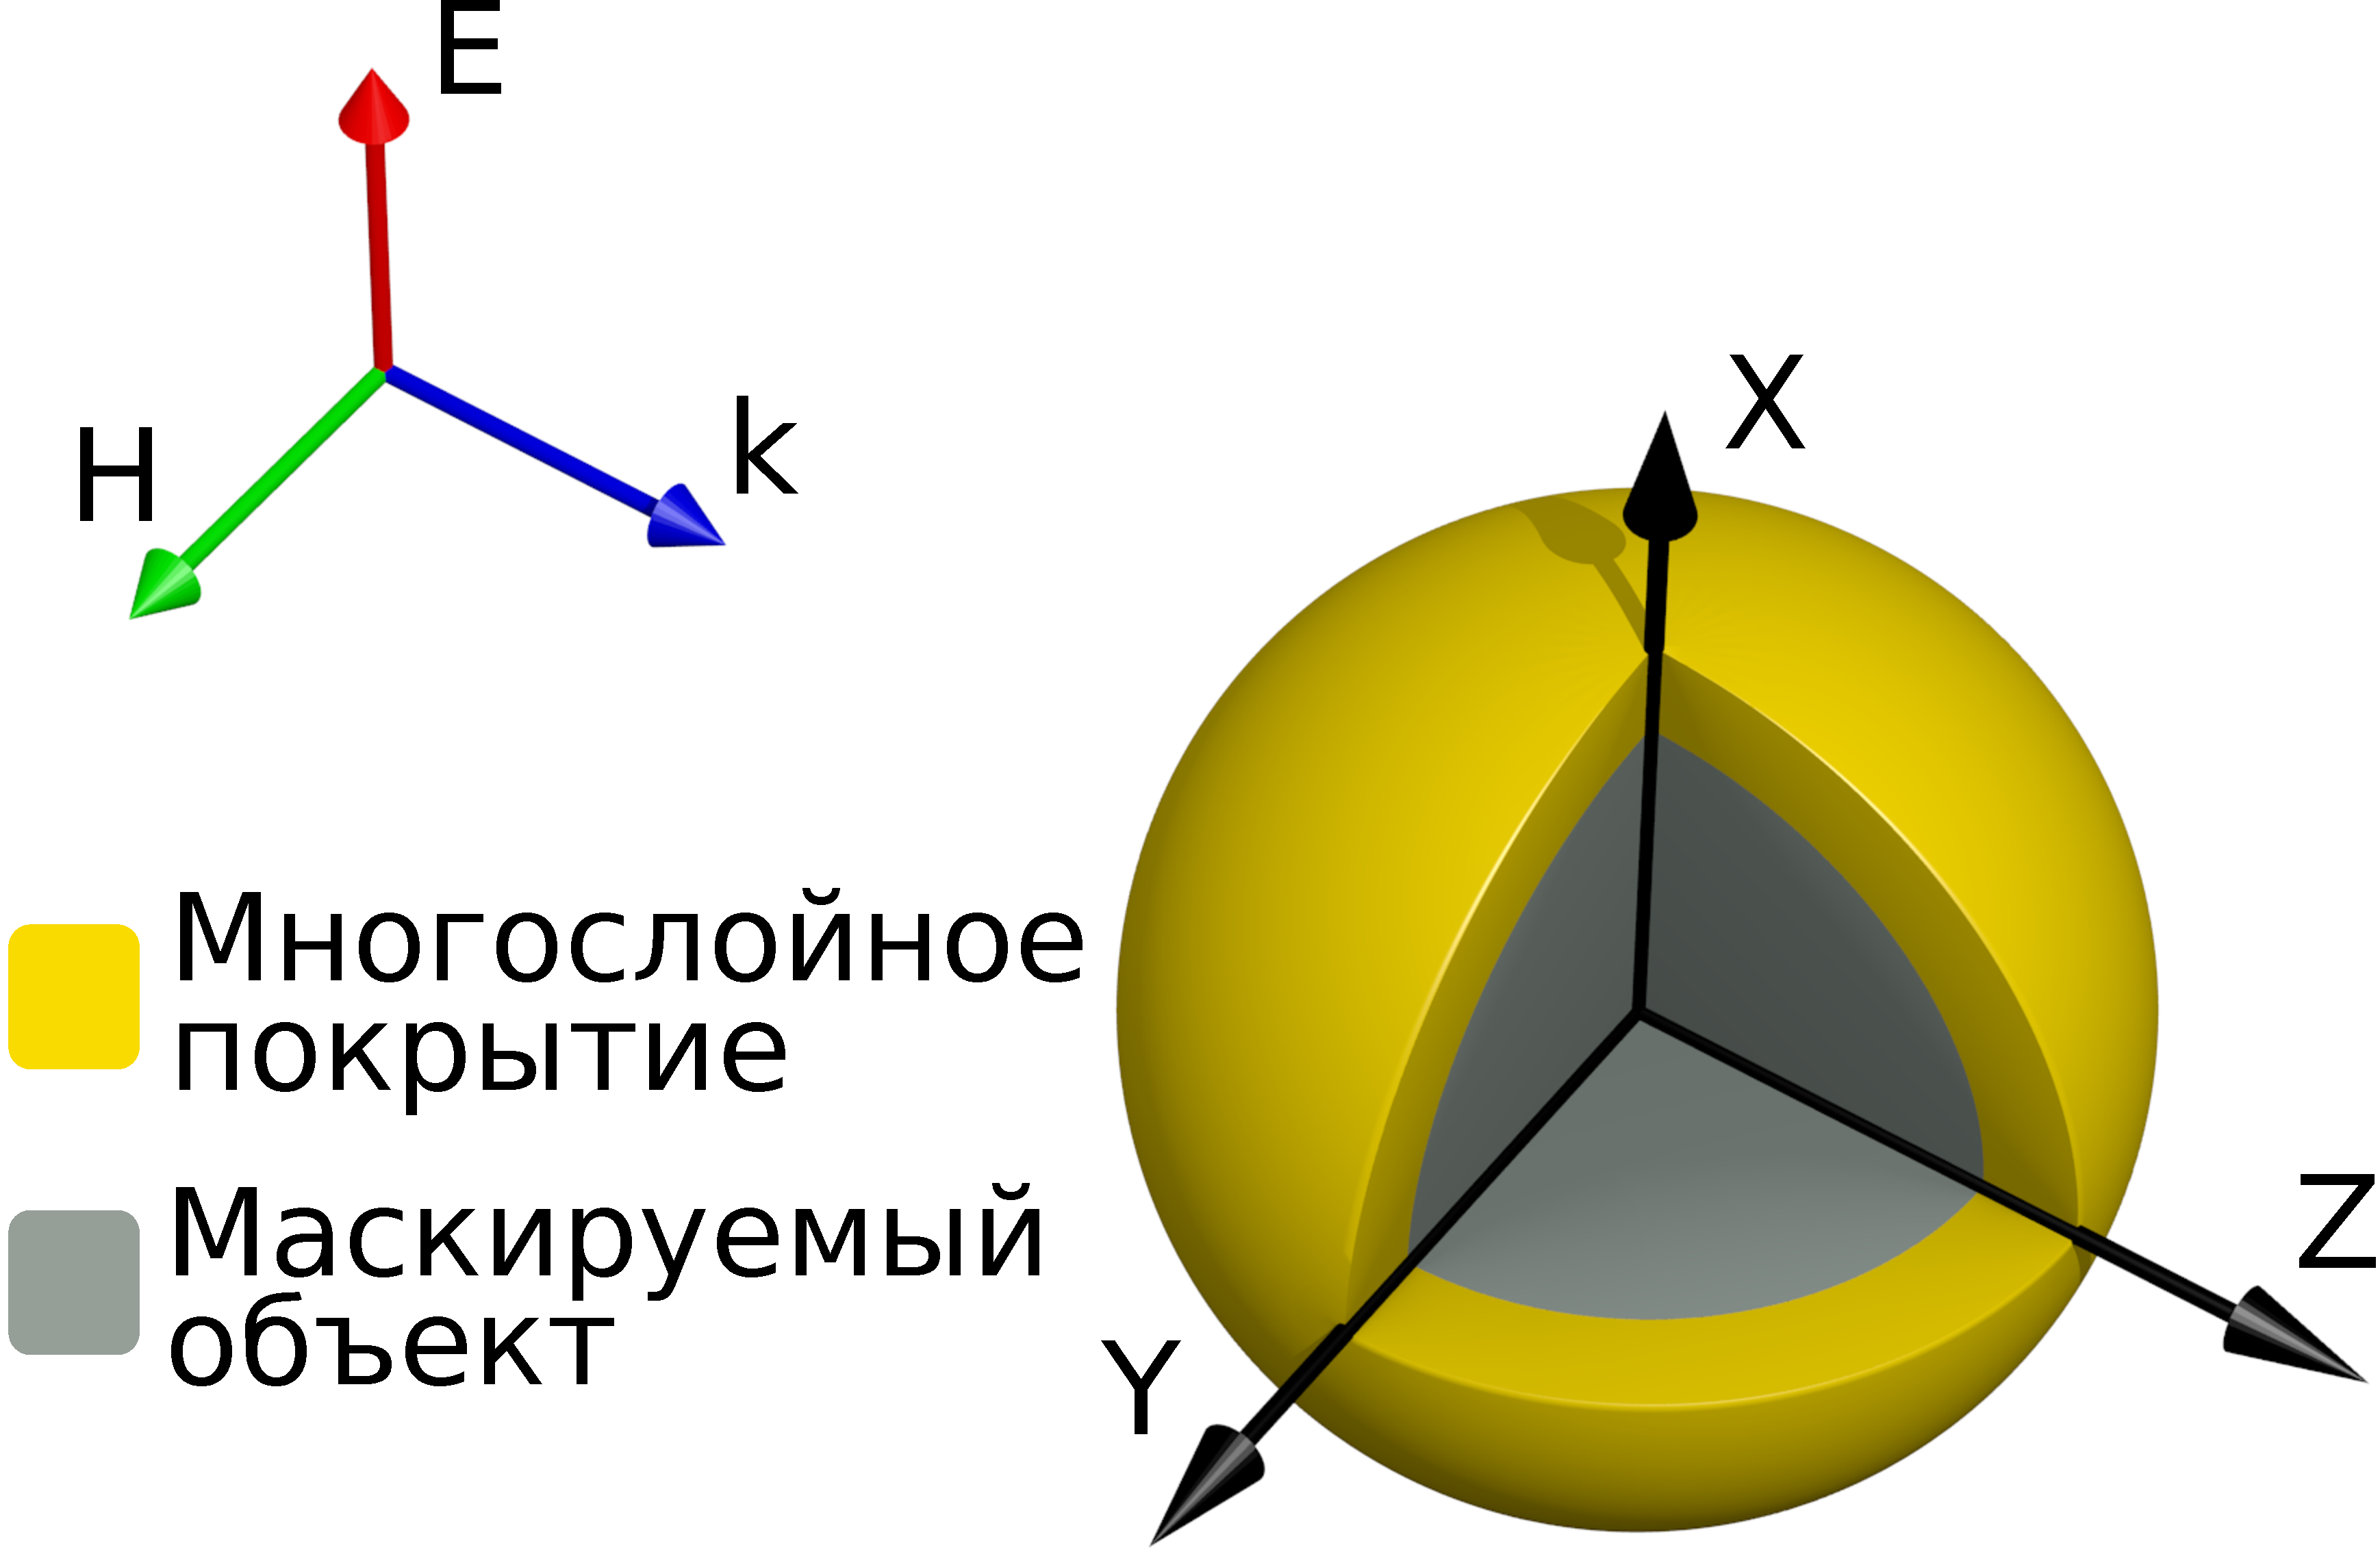
\includegraphics[width=0.95\linewidth]{model-view}}
  \end{minipage}
  \hfill
  \begin{minipage}[ht]{0.54\linewidth}
    \center{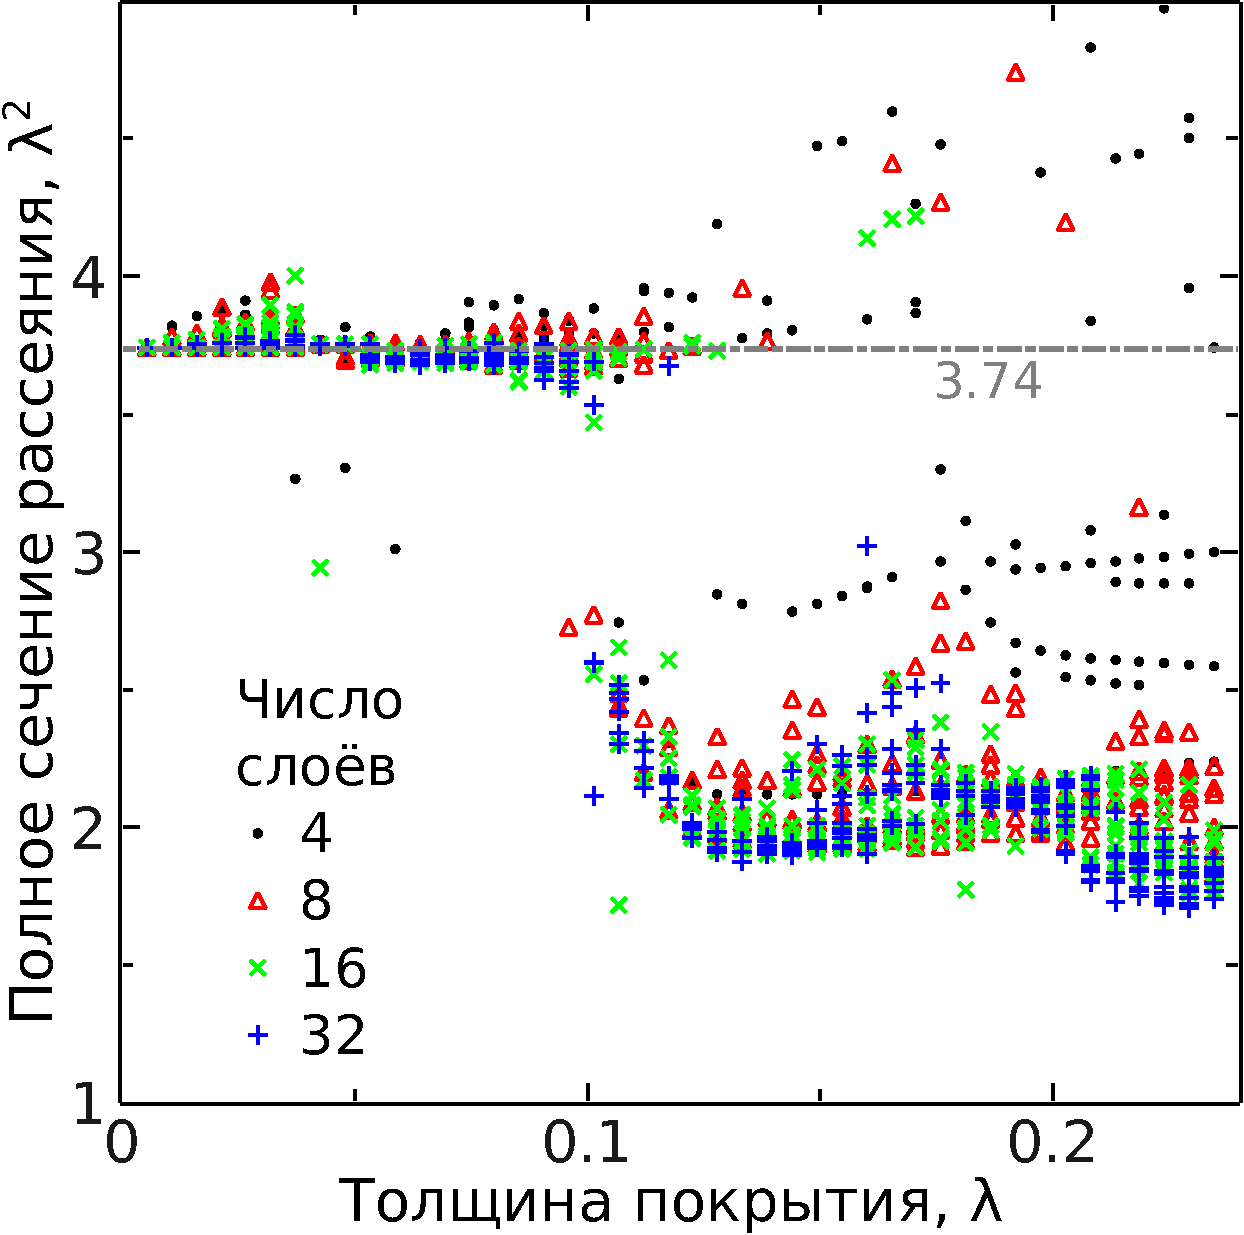
\includegraphics[width=0.95\linewidth]{rcs-overview} }
  \end{minipage}\\
  \vspace{0.3em}\\
  \begin{minipage}[ht]{0.45\linewidth}        
    \center{а)}
  \end{minipage}
  \hfill
  \begin{minipage}[ht]{0.54\linewidth}
    \center{б)}
  \end{minipage}

  \caption{(a) Схематическое изображение изучаемой системы: маскируемый
    объект -- сфера из идеального проводящего материала внутри
    многослойного диэлектрического покрытия и падающая
    электромагнитная волна. (б) 
    Результат работы оптимизатора для объекта диаметром $1.5\lambda$.
    % (TODO use plot for $\lambda/1.5$?)
    Каждая отметка на графике соответствует одному дизайну покрытия,
    полученному в результате минимизации рассеяния. При толщение
    покрытия $>0.15\lambda$ рассеяние можно уменьшить в $\sim 2$
    раза.}
  \label{img:scattering}  
\end{figure}
\begin{figure}[p]
  \begin{minipage}[ht]{0.32\linewidth}
    \center{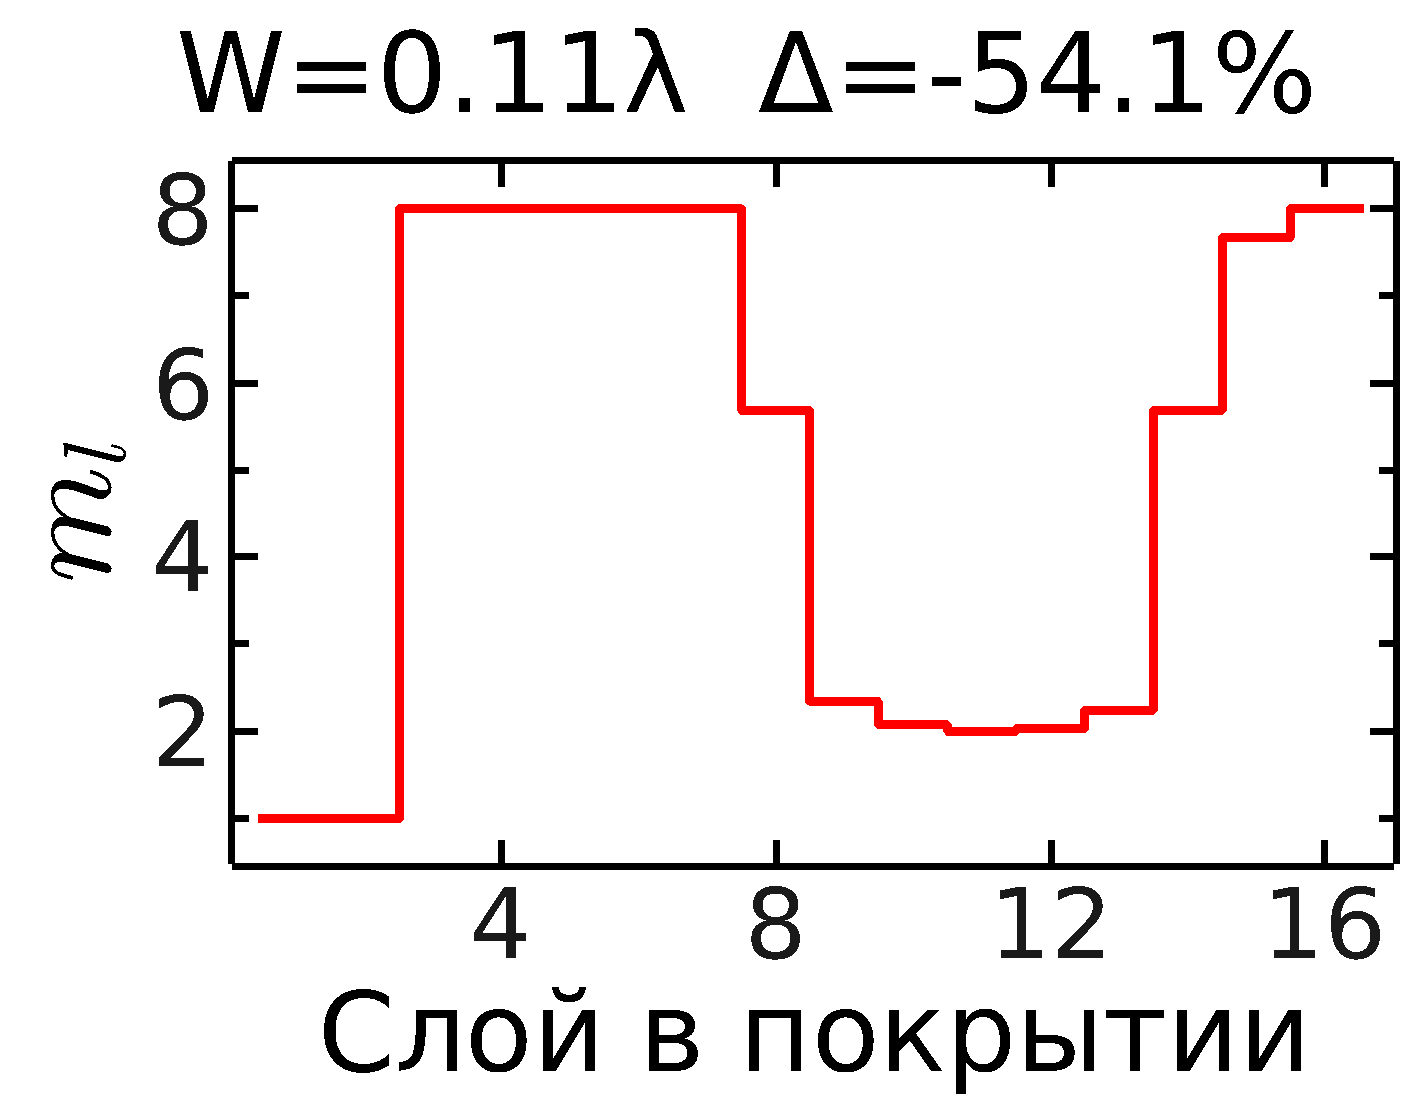
\includegraphics[width=0.95\linewidth]{w04-single-valley-index} \\ а)}
  \end{minipage}
  \hfill
  \begin{minipage}[ht]{0.32\linewidth}
    \center{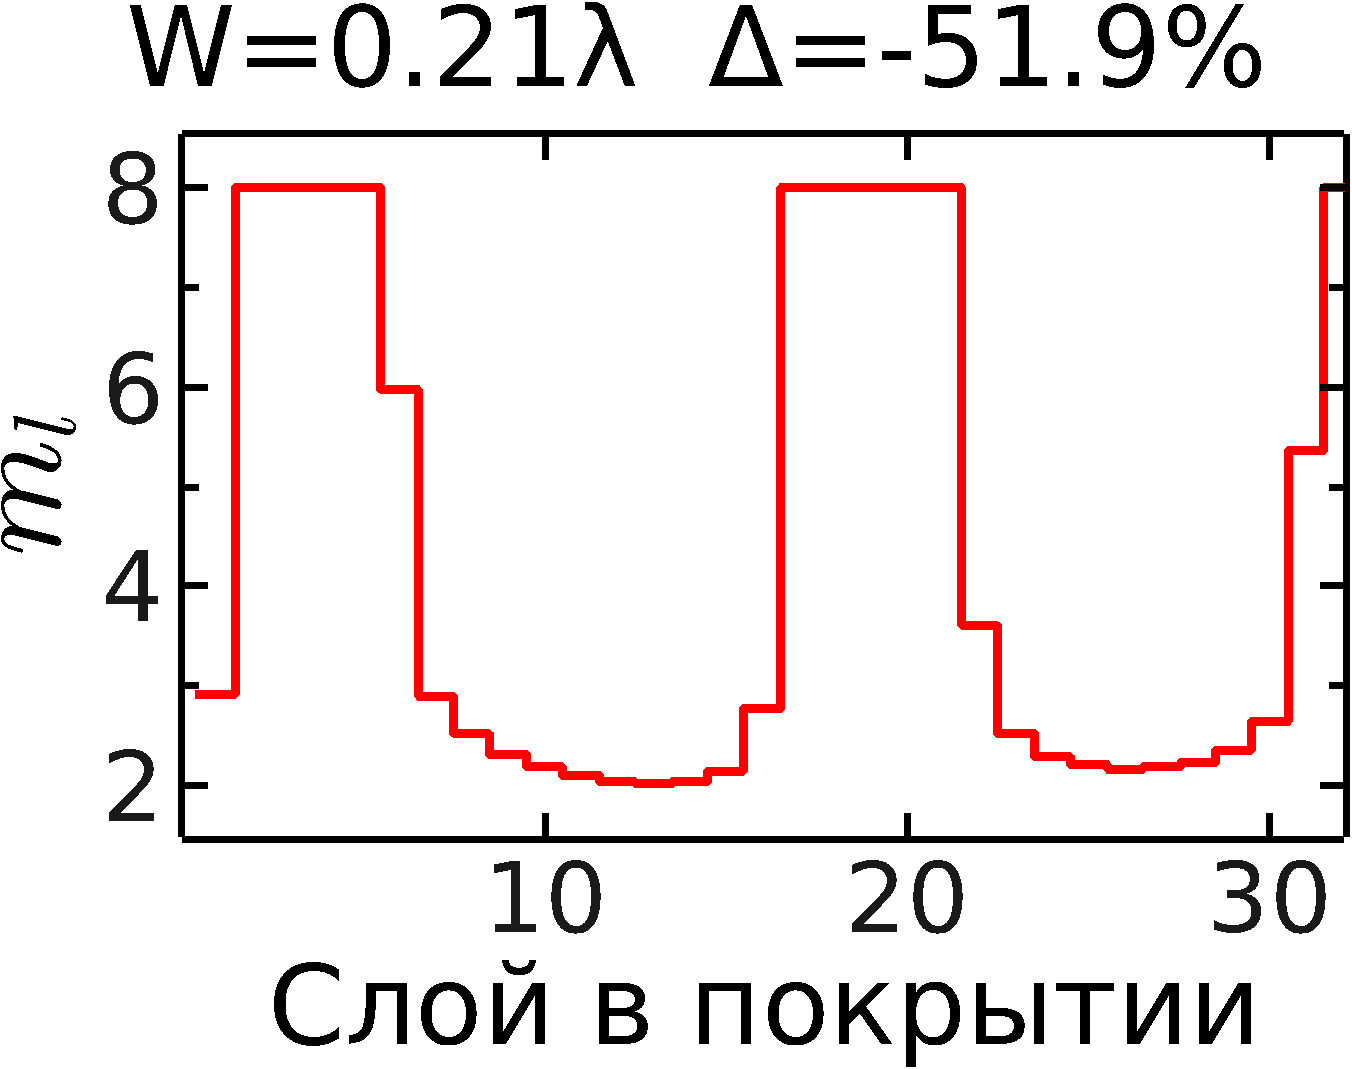
\includegraphics[width=0.95\linewidth]{w08-double-valley-index} \\ б)}
  \end{minipage}
  \hfill
  \begin{minipage}[ht]{0.32\linewidth}
    \center{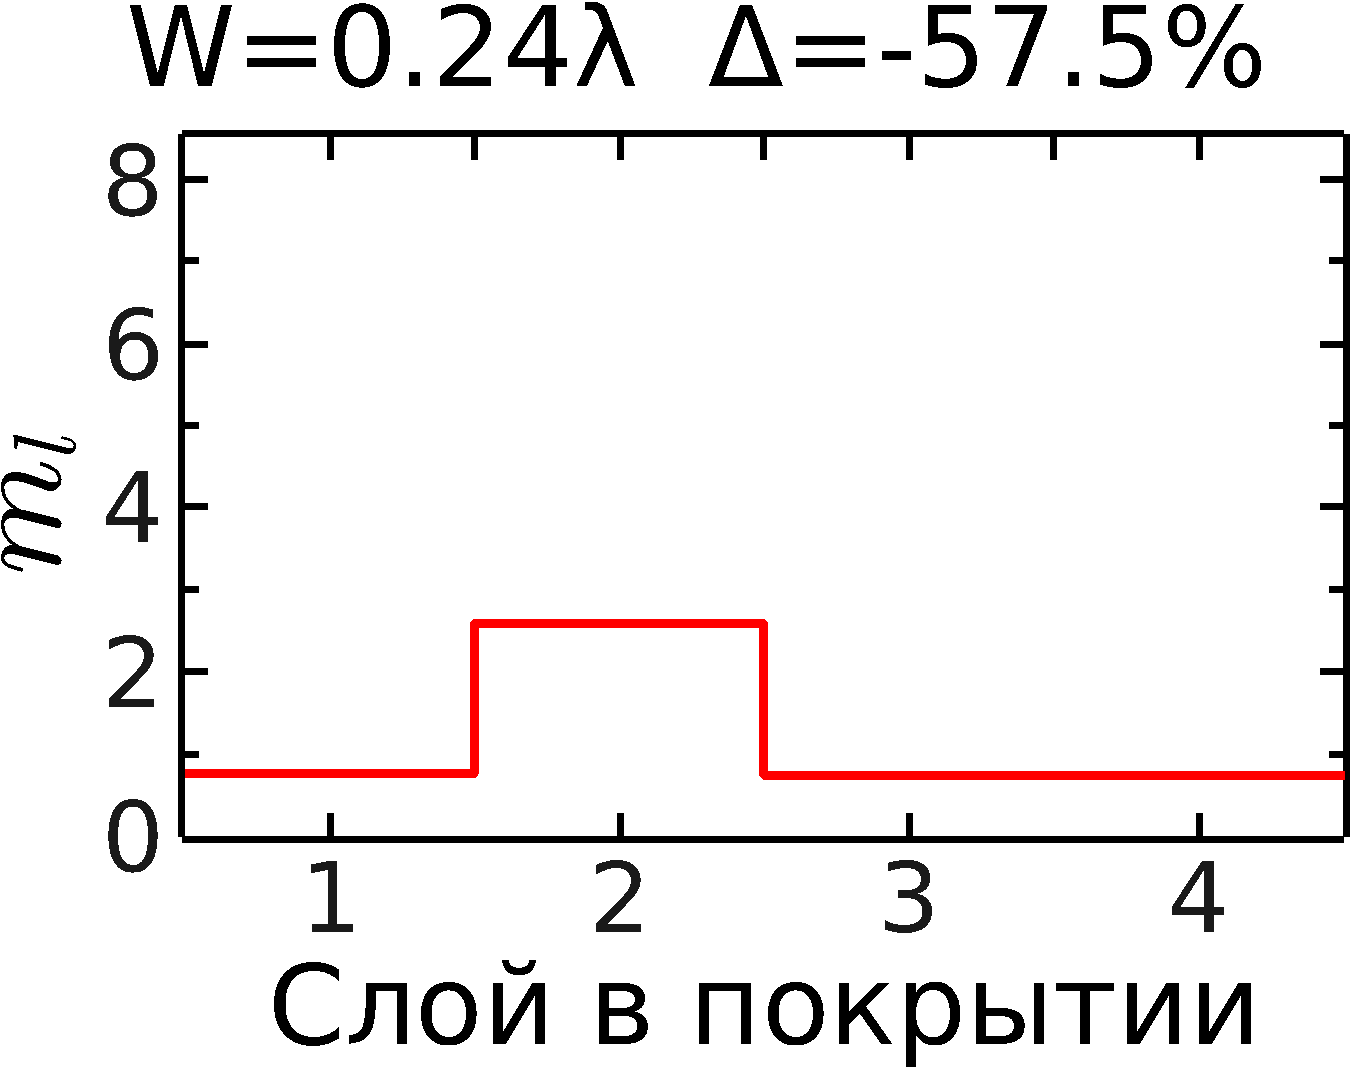
\includegraphics[width=0.95\linewidth]{index07-TO} \\ в)}
  \end{minipage}
  \caption{Типичные дизайны, обеспечивающие наилучшую маскировку при
    толщине покрытия равного (a)~$0.11\lambda$, (б)~$0.21\lambda$ и
    (в)~$0.24\lambda$. Максимальное значение показателя преломления
    было ограничено $n_{\rm max}=8$, а минимальное значение было равно
  (а,б) $n_{\rm min}=1$ и (в) $n_{\rm min}=0.67$}
  \label{img:designs}  
\end{figure}
\begin{figure}[p]
  \begin{minipage}[ht]{0.495\linewidth}
    \center{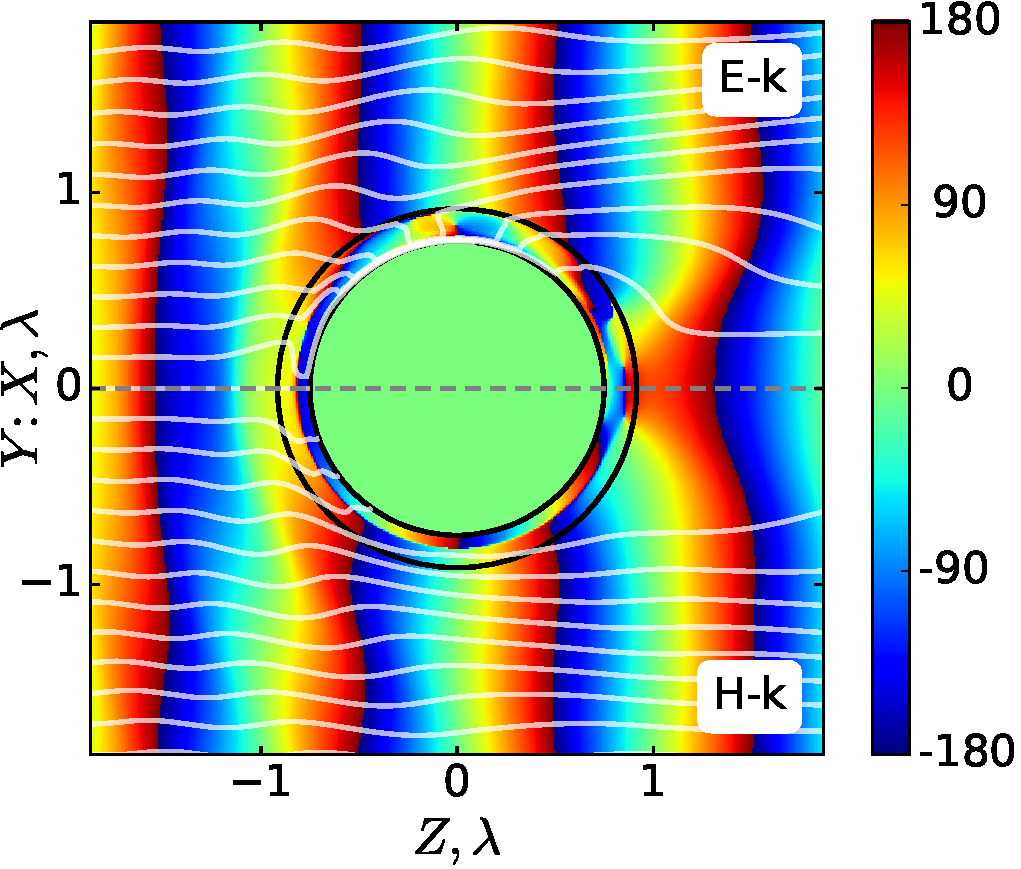
\includegraphics[width=0.98\linewidth]{PEC-index-sv-R3-XYZ-angleEx} \\ а)}
  \end{minipage}
  \hfill
  \begin{minipage}[ht]{0.495\linewidth}
    \center{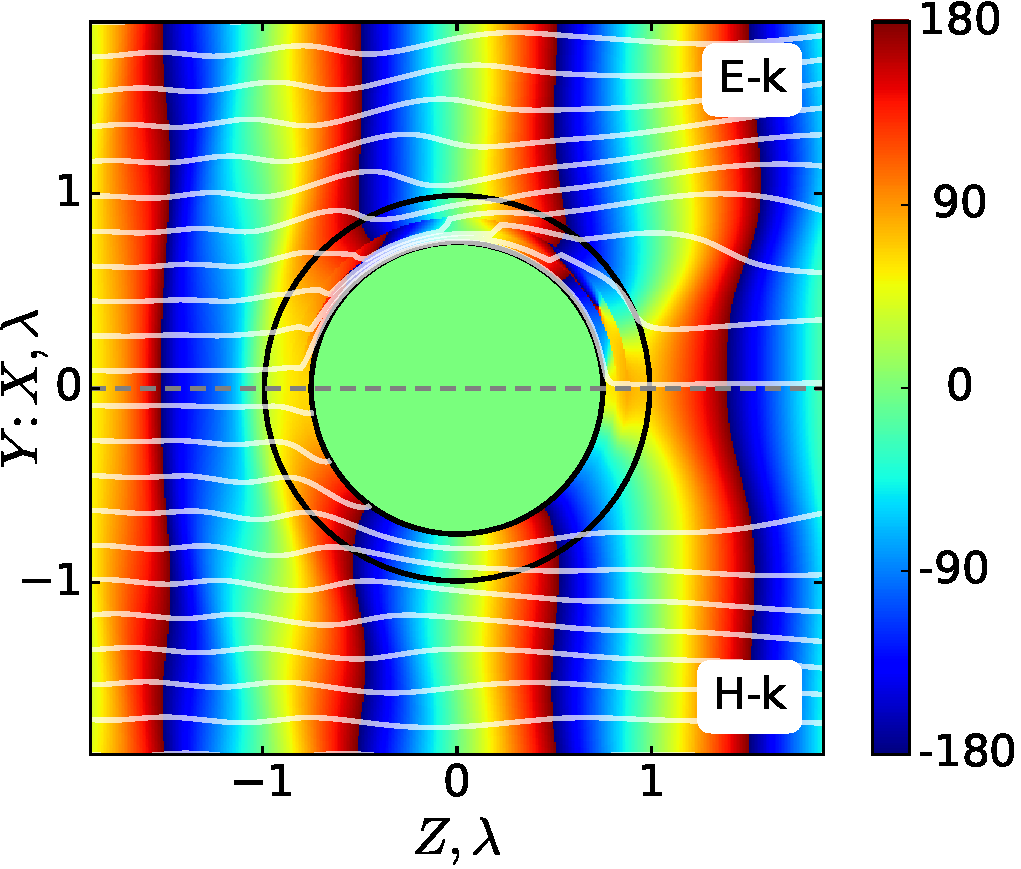
\includegraphics[width=0.98\linewidth]{PEC-index-in-glass-R1-XYZ-angleEx} \\ б)}
  \end{minipage}
  \caption{Изображение фазы электрического поля в случае маскировки
    объекта покрытием из изотропных (а) диэлектриков
    (см.~рисунок~\ref{img:designs}а) и (б) материалов с
    ${\varepsilon <1}$ (см.~рисунок~\ref{img:designs}в). Изображения
    построены в виде эпюра из плоскости поляризации падающей волны
    (верхняя половина) и перпендикулярной плоскости (нижняя
    половина). Чёрные окружности маркируют границы маскирующего
    покрытия. Белым обозначены линии потока энергии, волна
    распространяется в плоскости рисунка слева направо.}
  \label{img:field-phase}  
\end{figure}

Анализ этого и аналогичных графиков для других значений отношения
радиуса к длине волны позволил выявить ряд характерных
особенностей. Например, существует некое пороговое значение толщины,
после которого становится возможным стабильное получение дизайнов,
обеспечивающих заметное уменьшение сечения рассеяния. При этом
наилучшие показатели обеспечивают дизайны характерной структуры, где
несколько слоёв с высоким показателем преломления окружают группу
слоёв с низким показателем преломления. Увеличение общей толщины
покрытия приводит к переходу от дизайнов в одной такой группой
(рисунок~\ref{img:designs}а) к дизайнам с двумя группами
(рисунок~\ref{img:designs}б).

% ГОСТ Р 7.0.11—2011
% 5.3.9 На все иллюстрации должны быть приведены ссылки в тексте
% диссертации. При ссылке следует писать слово «Рисунок» с указанием
% его номера.

Сильной стороной теории Ми является возможность получать распределение
электрического и магнитного поля, как внутри, так и вокруг изучаемой
наночастицы, а также вычислять значение фазы полей и строить линии
потока энергии.  Например, для структуры, изображенной на
рисунке~\ref{img:designs}а, было рассчитано распределение фазы
электрического поля в окружающем частицу пространстве и внутри
покрытия (рисунок~\ref{img:field-phase}а).  Из рисунка видно, что
волна, проходящая через маскирующее покрытие, испытывает задержку фазы
приблизительно равную $2\pi$. Другими словами, такой дизайн приводит к
тому, что электромагнитная волна после распространения внутри покрытия
на выходе оказывается в фазе с волной, которая двигалась в окружающем
пространстве.  Это, в свою очередь, подавляет картину интерференции в
дальнем поле и, в конечном итоге, объясняет возникающий маскирующий
эффект.

Иначе выглядит распределение фазы электрического поля на
рисунке~\ref{img:field-phase}б, тут волна внутри покрытия на всей его
протяженности движется в фазе с волной в окружающем пространстве. Это
стало возможным из-за использования в оптимизации материалов с
${\varepsilon<1}$, что соответствует маскировке объекта во вмещающей
среде, в которой скорость распространения света ниже, чем внутри
маскирующего покрытия.  Такие покрытия отличаются характерным дизайном
(рисунок~\ref{img:designs}в), в котором один слой с высоким
показателем преломления находится между слоями с ${\varepsilon<1}$.
\begin{figure}[t]
  \begin{minipage}[ht]{0.49\linewidth}
    \center{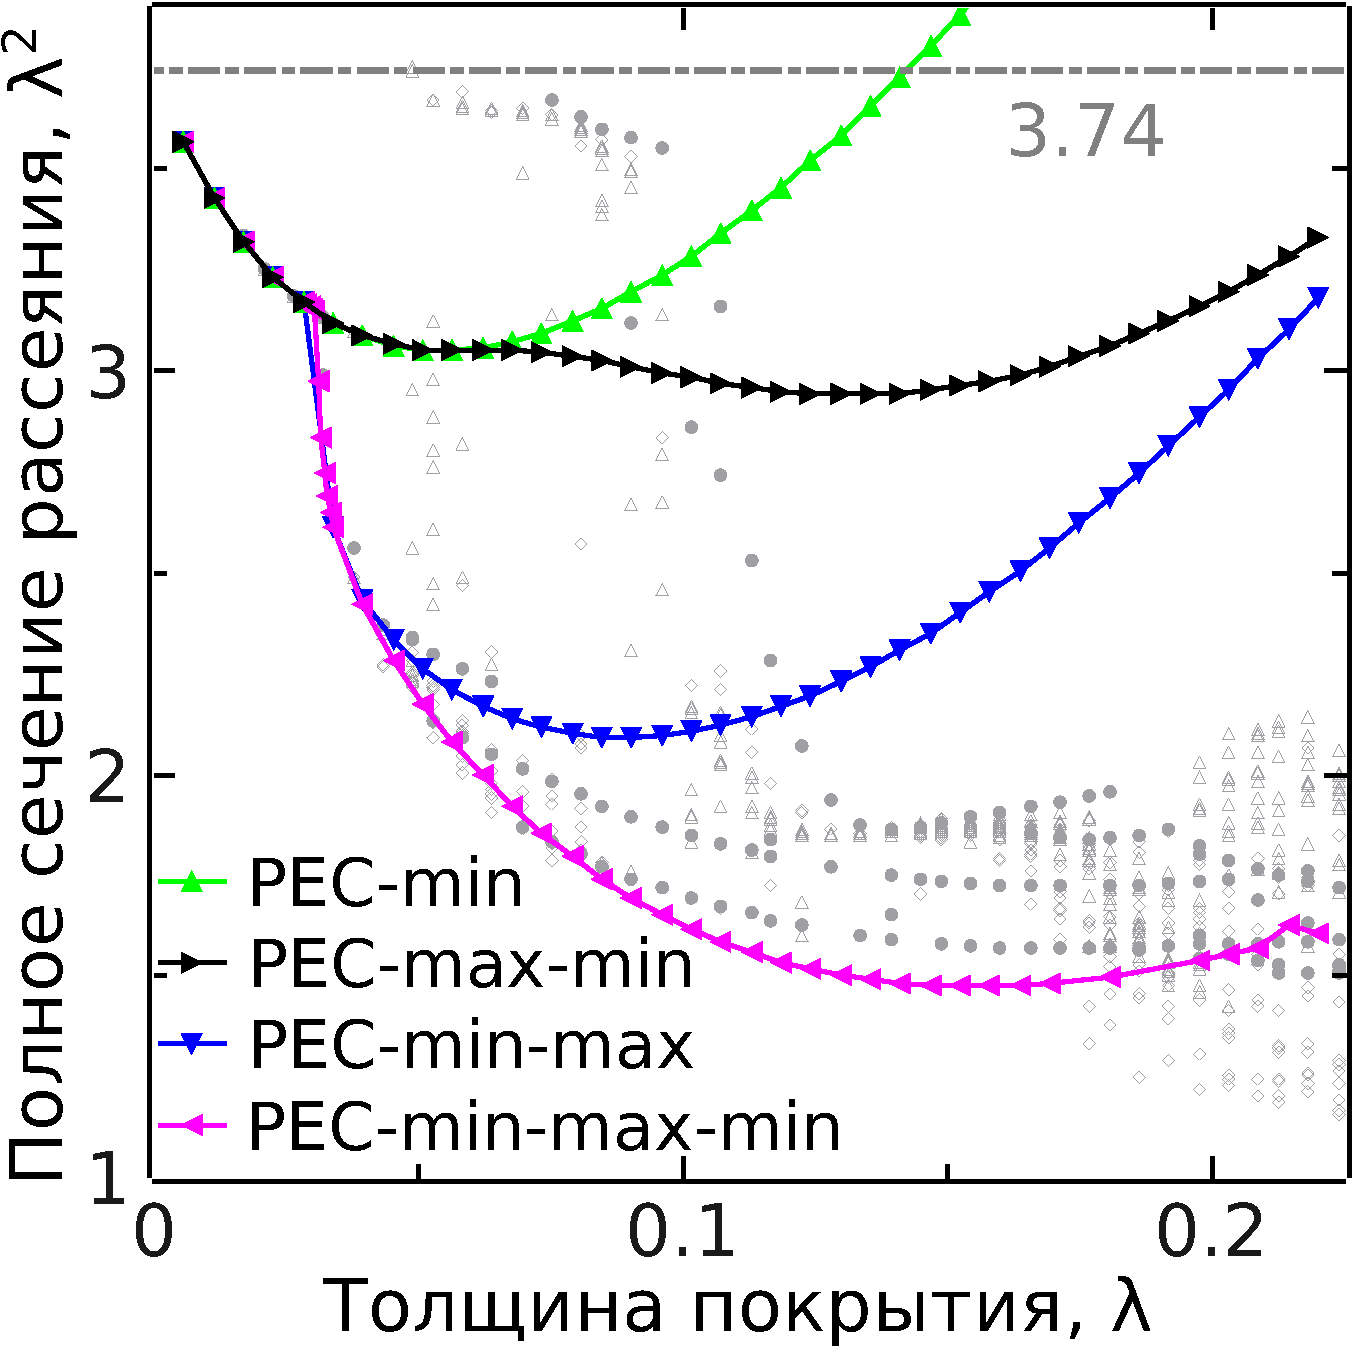
\includegraphics[width=0.95\linewidth]{rcs-overview-index07-DI} \\ а)}
  \end{minipage}
  \hfill
  \begin{minipage}[ht]{0.49\linewidth}
    \center{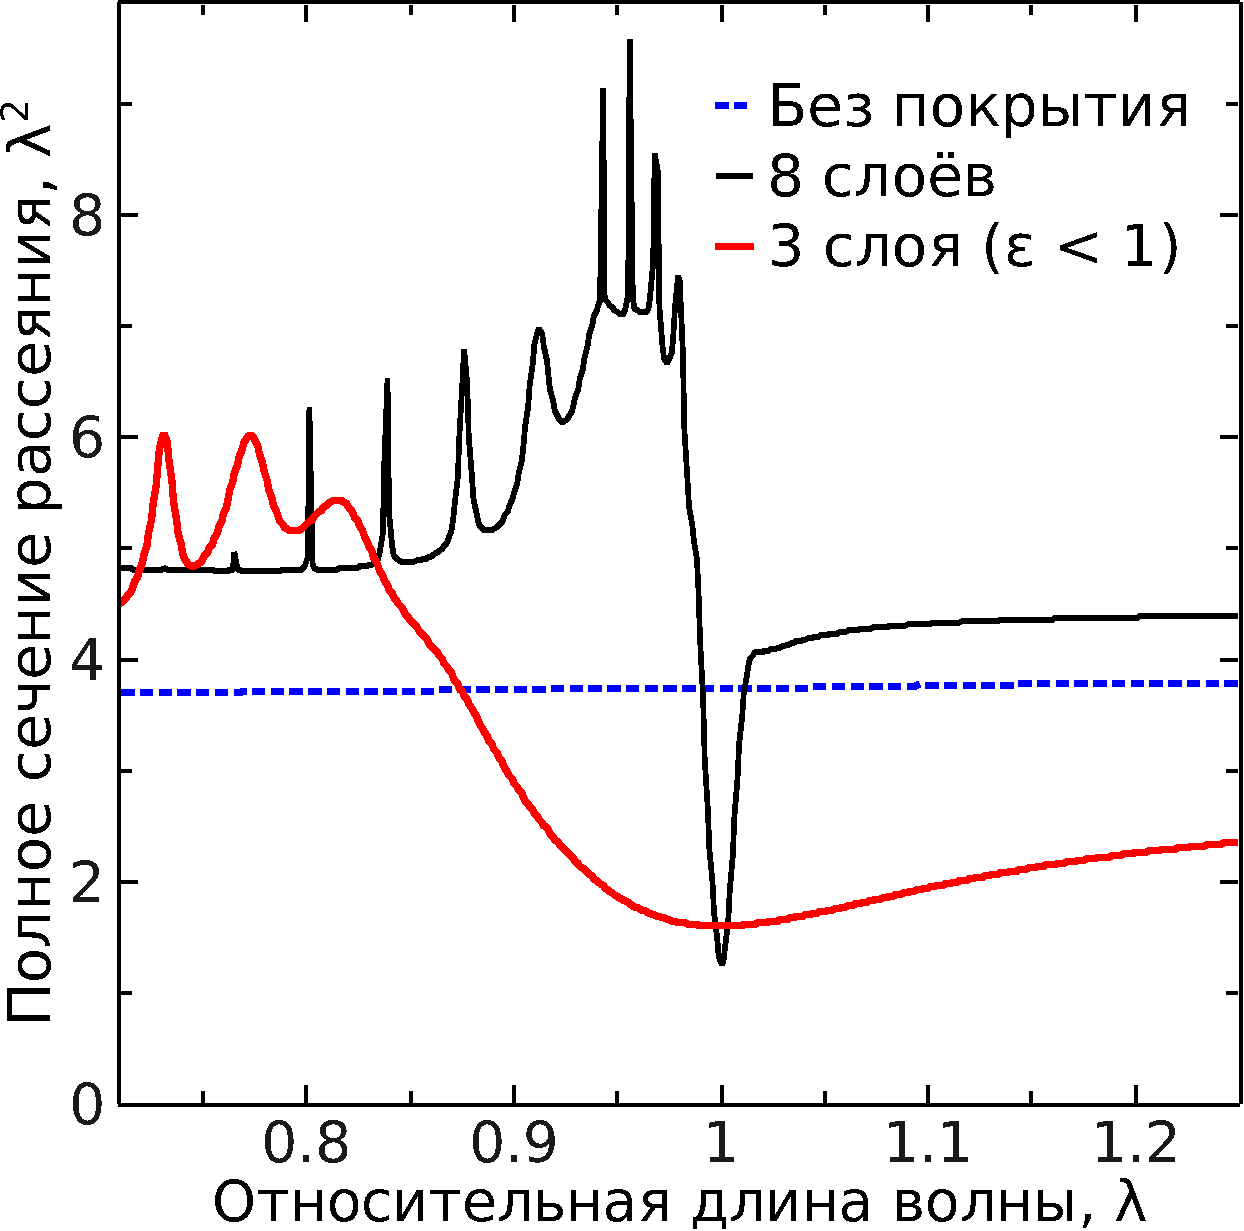
\includegraphics[width=0.95\linewidth]{index07-spectra} \\ б)}
  \end{minipage}
  \caption{а) Результат оптимизации покрытий с чередующимися слоями из
    большого $\varepsilon$ и ${\varepsilon<1}$. б) Спектры частицы
  без покрытия и с маскирующими покрытиями: из 8-ми слоёв диэлектрика и
  из 3-х слоёв с применением ${\varepsilon<1}$.}
  \label{img:min-max-min}  
\end{figure}

Обнаруженная закономерность позволила сформулировать гипотизу о том,
что для создания маскирующего покрытия достаточно использовать всего
два материала: с большим $\varepsilon$ и ${\varepsilon<1}$, а в
качестве параметров оптимизации можно использовать толщину каждого
слоя. Эта гипотеза была проверена численно, результаты оптимизации
отображены на рисунке~\ref{img:min-max-min}а. Оказалось, что для
большей части рассматриваемого диапазона общей толщины покрытия 
достаточно всего трёх слоёв, чтобы получить приблизительно то же
уменьшение полного сечения рассеяния, что и в случае применения 4, 8 и
16 слоёв равной толщины, когда в качестве параметров оптимизации
использовались материальные параметры каждого слоя.

Особый интерес представляет различие в спектрах рассеяния для случаев
наличия и отсутствия материала с ${\varepsilon<1}$ в оптимизированном
покрытии.  При расчёте спектров для рисунка~\ref{img:min-max-min}б не
учитывалось наличие в материалах дисперсии и сопутствующих потерь,
поэтому их форма полностью определяется дизайном маскирующего
покрытия. Хорошо виден относительно узкий резонанс, который определяет
маскирующие свойства покрытия на основе диэлектриков. Использование
материала с ${\varepsilon<1}$ позволило в несколько раз расширить
диапазон длин волн, где наблюдается подавление рассеяния. 

% 3-я глава 5 страниц. Общий объем 25 страниц.
% TODO в четвертую главу.

\underline{\textbf{В четвертой главе}} рассматривается явление
поглощения света многослойной наночастицей.

Достоинством теории Ми является используемое разложение поля по
сферическим векторным гармоникам, что позволяет разделить вклад в
общее поле от электрического и магнитного дипольного резонанса, а так
же вклад резонансов квадруполей и мультиполей более высокого
порядка. Таким образом, становится возможен покомпонентный анализ
спектрального отклика многослойной сферы в зависимости от её
дизайна. Например, в ряде случаев удаётся совместить в спектре
рассеяния положение нескольких резонансов (например, электрических
дипольного и квадрупольного), что создаёт эффект
суперрассеяния~\cite{Fan-2010,Fan-2011}. 

В настоящей работе был рассмотрен аналогичный эффект суперпоглощения
для наночастицы $Si/Ag/Si$, когда сечение поглощения сферической
наночастицы превышает фундаментальный предел поглощения резонансно
возбуждённого мультиполя максимального порядка. Ранее в своей
работе~\cite{Tribelsky-2011} М.И. Трибельский показал, что существует
верхний предел, ограничивающий возможности поглощения для одного
мультиполя, коэффициенты Ми для поглощения электрическими
$\tilde{a}_n= {\rm Re}\{a_n\} - |a_n|^2 $ и магнитными
$\tilde{b}_n= {\rm Re}\{b_n\} - |b_n|^2 $ модами не могут превысить
значения $1/4$.  При совмещении нескольких резонансов становится
возможным преодолеть этот фундаментальный предел. В этом случае
сечение поглощения оказывается больше, чем у однородной частицы того
же размера из произвольного изотропного материала.

При исследовании поглощения света наночастицами исследовались
трёхслойные частицы из заранее выбранных материалов, поэтому в
качестве параметров оптимизации использовались толщины составных
слоёв.  Целью оптимизации было получение структур с максимальной
эффективностью поглощения $Q_{\rm sca} = C_{\rm abs}/\pi R^2$ для
заданной длины волны, где $C_{\rm abs}$ это сечение поглощения, а $R$
это внешний радиус наночастицы.  Результат оптимизации для различных
значений $R$ представлен на рисунках~\ref{img:q-abs}(а-в). На
рисунке~\ref{img:q-abs}(а) дополнительными пунктирными линиями
отмечены максимально достижимые эффективности поглощения для
дипольного ($n=1$) и квадрупольного ($n=2$) резонансов выраженные в
виде~\cite{Tribelsky-2011}
$$Q^{(n)}_{\rm  abs\ max}=\frac{2n+1}{2q^2}$$
через параметр размера $q=2\pi R/\lambda$.  В рассматриваемой системе
максимальный порядок резонансного возбуждения мультиполей ограничен
квадруполем ($n=2$). Т.к. дизайны с внешним радиусом $R>60$~нм
демонстрируют эффективность поглощения выше, чем предел поглощения для
квадруполя, то, следовательно, выполняются условия для режима
суперпоглощения.

\begin{figure}[t]
  \begin{minipage}[ht]{0.495\linewidth}
    \center{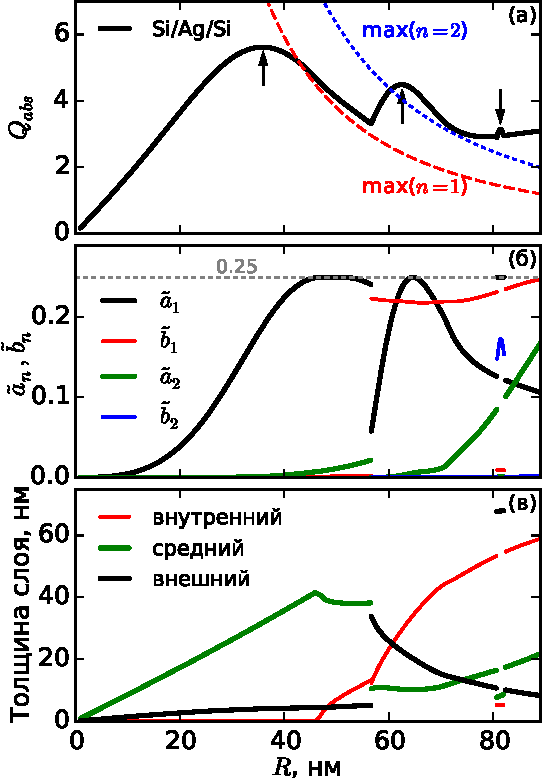
\includegraphics[height=1.35\linewidth]{2015-04-01-Qabs-SiAgSi-overview}}
  \end{minipage}
  \hfill
  \begin{minipage}[ht]{0.495\linewidth}
    \center{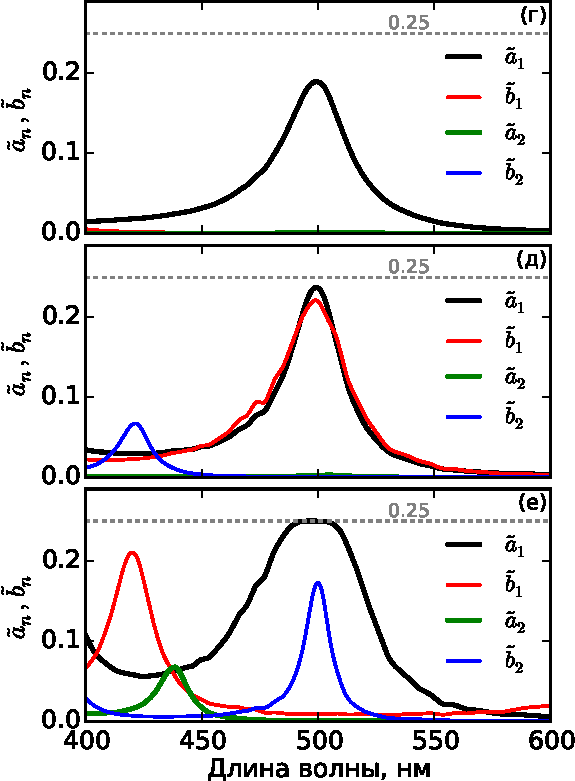
\includegraphics[height=1.35\linewidth]{2015-04-01-SiAgSi-ab-spectra4}}
  \end{minipage}
  \caption{ (а-в) Результат оптимизации эффективности поглощения
    $Si/Ag/Si$ наночастицей в зависимости от её внешнего радиуса, (а)
    эффективность поглощения, (б) коэффиценты поглощения в разложении
    Ми, где $\tilde{a}_1$ и $\tilde{a}_2$ относятся к электрическим, а
    $\tilde{b}_1$ и $\tilde{b}_2$ к магнитным диполю и квадруполю, (в)
    толщины составных слоёв наночастиц, (г-е) спектры коэффицентов
    поглощения в разложении Ми для дизайнов, соответствующих локальным
    максимумам на рисунке~\ref{img:q-abs}а.}
  \label{img:q-abs}  
\end{figure}


На рисунке~\ref{img:q-abs}(б) изображены значения коэффицентов Ми для
поглощения различными модами, горизонтальной пунктирной линией
отмечено значение теоретически достижимого предела для них, равное
1/4. В случае небольшого размера частицы основной вклад в поглощение
даёт электрический диполь $\tilde{a}_1$.  При оптимизации дизайнов для
$R > 56.6$~нм оказалось, что дизайны с поглощением на электрическом и
магнитном диполях позволяет достичь большего общего сечения
поглощения, чем в случае поглощения только электрическим
диполем. Такое качественное изменение соответствует разрывам линий на
рисунках~\ref{img:q-abs}(б-в) и реализует режим суперпоглощения.
Необходимо отметить, что для небольшого диапазона размеров частицы 
$80.7<R<82.1$~нм оптимальное поглощение обеспечивает использование
электрического дипольного $\tilde{a}_1$ и магнитного квадрупольного
$\tilde{b}_2$ резонансов, что приводит ещё к двум разрывам линий на
рисунках для соответствующих значений внешнего радиуса~$R$.

На рисунке~\ref{img:q-abs}(в) представлены толщины составных слоёв
наночастицы, полученные в результате оптимизации эффективности
поглощения.  Неожиданно оказалось, что дизайны с преобладающим
дипольным механизмом поглощения (т.е. для размеров частицы менее
56.6~нм) могут быть двух видов.  Чтобы получить наилучшее поглощение
для $R<46$~нм хватает использования всего двух слоёв, при оптимизации
толщина внутреннего слой исходного трёхслойного дизайна обратилась в
ноль.  При $R=46$~нм поглощение диплем почти достигает своего
теоретического предела ($\tilde{a}_1>0.249$), чтобы удерживать его
близи этого значения для больших значений $R$ оптимизатор начает
наращивать толщину внутреннего кремниевого слоя.  В свою очередь это
приводит к появлению слабого поглощения квадруполем $\tilde{a}_2$,
что, впрочем, не позволяет достичь режима суперпоглощения для $n=2$.

Для расчёта спектров на рисунках~\ref{img:q-abs}(г-е) были
использованы экспериментальные дисперсионные зависимости для
показателей преломления из работы\cite{palik-1997}. Спектры коэффицентов
поглощения в разложении Ми построены для дизайнов, соответствующих локальным
максимумам на рисунке~\ref{img:q-abs}(а). Спектр для дизайна с внешним
радиусом $R=36$~нм на рисунке~\ref{img:q-abs}(г) подтверждает дипольный характер поглощения с
резонансом на выбранной для оптимизации длины волны $\lambda=500$~нм.
Спектры дизайнов с максимумами поглощения для $R=63$~нм и $R=81$~нм
(рисунки~\ref{img:q-abs}(д) и~\ref{img:q-abs}(е) соответственно)
обладают типичной для суперпоглощения структрурой с вырождением
нескольких резонансов. На этих спектрах присутствуют дополнительные
резонансы, которые, впрочем, расположены в значительном отдалении от
выбранной для оптимизации длины волны, поэтому их вклад в общее
поглощение мал.

Особо надо отметить, что для получения максимальной эффективности
поглощения вовсе не требуется реализация режима суперпоглощения.  Из
рисунка~\ref{img:q-abs}(а) следует, что максимальная эффективность
соответствует малым размерам частицы, где значение коэффициента Ми для
поглощения заметно меньше теоретического предела. Среди всех
рассмотренных структур двухслойная частица $Ag/Si$ с внешним радиусом
36~нм обладает максимальной эффективностью поглощения. Для этой
частицы сечение поглощения более чем 5 раз превысило её геометрическое
сечение. Дополнительным преимуществом таких частиц может являться то,
что они должны быть проще и дешевле в производстве по сравнению с
трёхслойными.  В то же время для частиц большего размера ($R>60$~нм
для рассмотренных материалов) максимальная эффективность получается в
режиме суперпоглощения.  Это может оказаться существенно для случая,
когда изготовление многослойных частиц меньшего размера не доступно по
какой-либо технологической причине.



В \underline{\textbf{заключении}} приведены основные результаты
работы, которые заключаются в следующем: %% Согласно ГОСТ Р 7.0.11-2011:
%% 5.3.3 В заключении диссертации излагают итоги выполненного исследования, рекомендации, перспективы дальнейшей разработки темы.
%% 9.2.3 В заключении автореферата диссертации излагают итоги данного исследования, рекомендации и перспективы дальнейшей разработки темы.
\begin{enumerate}
  \item Предложен метод изучения экстремальных оптических свойств
    многослойных сферических наночастиц с помощью теории Ми и
    стохастической оптимизации. Высокая вычислительная
    производительность этого подхода позволила выявить несколько новых
    физических эффектов, связанных с рассеянием и поглощением
    электромагнитной волны на многослойных сферических наночастицах.
  \item В задаче рассеяния плоской волны на многослойной сфере
    получены явные рекуррентные соотношения для коэффициентов Ми в
    расчёте локальных полей, выраженные через логарифмические
    производные функций Риккати-Бесселя.  Эти соотношения были
    добавлены в компьютерную программу, выполняющую вычисления в
    рамках задачи Ми.
  \item Рассеяние от объекта из идеального проводника можно
    существенно уменьшить с помощью многослойного покрытия толщиной
    $0.15\lambda$, используя только изотропные диэлектрические
    материалы: в 2 и в 6 раз для объектов диаметром $1.5\lambda$ и
    $\lambda/1.5$ соответственно. Обнаружен пороговый характер
    уменьшения рассеяния в зависимости от толщины покрытия.
  \item % (TODO берем балошени без слов min-max-min)
    Среди разнообразных оптимизированных дизайнов маскирующих покрытий из
    изотропных материалов с $\varepsilon$ меньше единицы, состоящих из
    множества слоёв равной толщины, выявлена закономерность,
    позволяющая разрабатывать эффективные трёхслойные сферические
    покрытия с разными толщинами слоёв. Дополнительной особенностью
    таких покрытий является значительное увеличение области спектра, в
    которой наблюдается эффект маскировки, при сравнении с покрытиями
    из диэлектриков. 
    %%%%%% Спектр --- засада
  \item В трёхслойных частицах $Si/Ag/Si$ возможно вырождение
    мультипольных резонансов, приводящее к эффекту суперпоглощения,
    когда сечение поглощения оказывается больше, чем у однородной
    частицы того же размера из произвольного изотропного
    материала. Максимальная эффективность поглощения в
    рассматриваемой системе была получена для небольших двухслойных
    частиц с преобладающей ролью электрического дипольного резонанса.
\end{enumerate}



%\newpage
При использовании пакета \verb!biblatex! список публикаций автора по теме
диссертации формируется в разделе <<\publications>>\ файла
\verb!../common/characteristic.tex!  при помощи команды \verb!\nocite! 

\ifthenelse{\equal{\thebibliosel}{0}}{% Встроенная реализация с загрузкой файла через движок bibtex8
  \renewcommand{\refname}{\large \authorbibtitle}
  \nocite{*}
  \insertbiblioauthor                          % Подключаем Bib-базы
  %\insertbiblioother   % !!! bibtex не умеет работать с несколькими библиографиями !!!
}{% Реализация пакетом biblatex через движок biber
  \insertbiblioauthor                          % Подключаем Bib-базы
  \insertbiblioother
}

%%% Local Variables:
%%% mode: latex
%%% TeX-master: "../synopsis"
%%% End:
